\documentclass[landscape,a0paper,fontscale=0.292]{baposter}

\usepackage[vlined]{algorithm2e}
\usepackage{times}
\usepackage{calc}
\usepackage{url}
\usepackage{graphicx}
\usepackage{amsmath}
\usepackage{amssymb}
\usepackage{relsize}
\usepackage{multirow}
\usepackage{booktabs}

\usepackage{graphicx}
\usepackage{multicol}
\usepackage[T1]{fontenc}
\usepackage{ae}

\graphicspath{{images/}}

 % Multicol Settings
 \setlength{\columnsep}{0.7em}
 \setlength{\columnseprule}{0mm}


 % Save space in lists. Use this after the opening of the list
 \newcommand{\compresslist}{%
 \setlength{\itemsep}{1pt}%
 \setlength{\parskip}{0pt}%
 \setlength{\parsep}{0pt}%
 }

 % Formating
 \newcommand{\Matrix}[1]{\begin{bmatrix} #1 \end{bmatrix}}
 \newcommand{\Vector}[1]{\begin{pmatrix} #1 \end{pmatrix}}

 \newcommand*{\norm}[1]{\mathopen\| #1 \mathclose\|}% use instead of $\|x\|$
 \newcommand*{\abs}[1]{\mathopen| #1 \mathclose|}% use instead of $\|x\|$
 \newcommand*{\normLR}[1]{\left\| #1 \right\|}% use instead of $\|x\|$

 \DeclareMathOperator*{\argmax}{arg\,max}
 \DeclareMathOperator*{\diag}{diag}
 \DeclareMathOperator*{\argmin}{arg\,min}
 \DeclareMathOperator*{\vectorize}{vec}
 \DeclareMathOperator*{\reshape}{reshape}

 % Koerper
 \font\dsfnt=dsrom12
 \DeclareSymbolFont{nark}{U}{dsrom}{m}{n}

\begin{document}
\begin{poster}{
    % Show grid to help with alignment
    grid=false,
    % Column spacing
    colspacing=0.7em,
    % Color style
    headerColorOne=cyan!20!white!90!black,
    borderColor=cyan!30!white!90!black,
    % Format of textbox
    textborder=faded,
    % Format of text header
    headerborder=open,
    headershape=roundedright,
    headershade=plain,
    background=none,
    bgColorOne=cyan!10!white,
    headerheight=0.12\textheight
}
 % Eye Catcher
 {
      \includegraphics[width=0.08\linewidth]{track_frame_00010_06}
      \includegraphics[width=0.08\linewidth]{track_frame_00450_06}
      \includegraphics[width=0.08\linewidth]{track_frame_04999_06}
 }
 % Title
 {\sc\Huge On Compositional Image Alignment}
 % Authors
 {Brian Amberg, Andrew Blake, and Thomas Vetter\\[1em]
 {\texttt{Brian.Amberg@unibas.ch, ab@microsoft.com, Thomas.Vetter@unibas.ch}}}
 % University logo
 {
  \begin{tabular}{r}
    \includegraphics[height=0.12\textheight]{logo}\\
    \raisebox{0em}[0em][0em]{\includegraphics[height=0.03\textheight]{msrlogo}}
  \end{tabular}
 }

%%%%%%%%%%%%%%%%%%%%%%%%%%%%%%%%%%%%%%%%%%%%%%%%%%%%%%%%%%%%%%%%%%%%%%%%%%%%%%
%%% Now define the boxes that make up the poster
%%%---------------------------------------------------------------------------
%%% Each box has a name and can be placed absolutely or relatively.
%%% The only inconvenience is that you can only specify a relative position 
%%% towards an already declared box. So if you have a box attached to the 
%%% bottom, one to the top and a third one which should be inbetween, you 
%%% have to specify the top and bottom boxes before you specify the middle 
%%% box.
%%%%%%%%%%%%%%%%%%%%%%%%%%%%%%%%%%%%%%%%%%%%%%%%%%%%%%%%%%%%%%%%%%%%%%%%%%%%%%

%%%%%%%%%%%%%%%%%%%%%%%%%%%%%%%%%%%%%%%%%%%%%%%%%%%%%%%%%%%%%%%%%%%%%%%%%%%%%%
  \headerbox{Contribution: Fast \emph{and} reliable Face Alignment}{name=contribution,column=0,row=0,span=2}{
%%%%%%%%%%%%%%%%%%%%%%%%%%%%%%%%%%%%%%%%%%%%%%%%%%%%%%%%%%%%%%%%%%%%%%%%%%%%%%
  Inverse compositional image alignment (ICIA) is fast, but not reliable. We
  explain ICIA from a different perspective which leads naturally to two new
  algorithms with a better capture range and comparable speed.
  }
%%%%%%%%%%%%%%%%%%%%%%%%%%%%%%%%%%%%%%%%%%%%%%%%%%%%%%%%%%%%%%%%%%%%%%%%%%%%%%
  \headerbox{There is no \emph{inverse} in \emph{ICIA}}{name=abstract,column=0,below=contribution}{
%%%%%%%%%%%%%%%%%%%%%%%%%%%%%%%%%%%%%%%%%%%%%%%%%%%%%%%%%%%%%%%%%%%%%%%%%%%%%%
    Image aligment minimizes
    \begin{align}
      \F{\qq} &\defined \normLR{ \e{\qq,\pb} }^2_{\D},\label{eqn:f}\\
    \text{with }  \e{\qq} &\defined a - I\circ \W{\qq}\nonumber
    \end{align}
    composition with an incremental warp $\Vs$ approximates $\Fs$ around $\qq_0$ as
    \begin{align}
      \F{\C{\circ}{\qq_0, \pp}} \approx \FF{\qq_0, \pp} & \defined \normLR{\ee{\qq_0,\pp}}^2_{\D}\label{eqn:comp}\\
      \text{with } \ee{\qq_0, \pp}&\defined  \INTf(a -  I \circ \W{\qq_0} \circ \V{\pp}) \quad.\nonumber
    \end{align}
    The gradient descent or Gauss-Newton update rule then gives an estimate of
    the incremental warp, which drives the model warp.

    ICIA can be derived by substituting the current backwarped image with the
    model appearance after taking the derivative. The substitution can be used
    to get an approximate gradient and/or Hessian, leading to a family of
    algorithms.

    Additionally we replace the incremental warp $V$ with an orthonormalized
    warp and regularize in the composition step. The result is a vast
    improvement in robustness without sacrificing speed.
}



 %%%%%%%%%%%%%%%%%%%%%%%%%%%%%%%%%%%%%%%%%%%%%%%%%%%%%%%%%%%%%%%%%%%%%%%%%%%%%%
   \headerbox{Our methods are at the performance/speed sweet point}{name=speed,column=2,row=0,span=2}{
 %%%%%%%%%%%%%%%%%%%%%%%%%%%%%%%%%%%%%%%%%%%%%%%%%%%%%%%%%%%%%%%%%%%%%%%%%%%%%%
   \newlength{\MSZ}
   \setlength{\MSZ}{0.01\textwidth}
   \newcommand{\MarkerCircle}[1]{%
     \tikz{\draw[use as bounding box] (0,0); \draw[fill=#1]             circle(\MSZ);}}
   \newcommand{\MarkerRectangle}[1]{%
     \tikz{\draw[use as bounding box] (0,0); \draw[fill=#1]             (-\MSZ,-\MSZ) rectangle +(2\MSZ,2\MSZ);}}
   \newcommand{\MarkerDiamond}[1]{%
     \tikz{\draw[use as bounding box] (0,0); \draw[fill=#1,rotate=45]   rectangle +(2\MSZ,2\MSZ);}}
   \newcommand{\MarkerTriangle}[1]{%
     \tikz{\draw[use as bounding box] (0,0); \draw[fill=#1]             (-0.866\MSZ,-0.5\MSZ) -- (0\MSZ,1\MSZ) -- (0.866\MSZ,-0.5\MSZ) -- cycle ;}}
   \newcommand{\MarkerUDTriangle}[1]{%
     \tikz{\draw[use as bounding box] (0,0); \draw[fill=#1,rotate=180]  (-0.866\MSZ,-0.5\MSZ) -- (0\MSZ,1\MSZ) -- (0.866\MSZ,-0.5\MSZ) -- cycle ;}}
   \newcommand{\MarkerPlus}[1]{%
     \tikz{\draw[use as bounding box] (0,0); \draw[fill=#1]         (-\MSZ,-0.25\MSZ) rectangle +(2\MSZ,0.5\MSZ) (-0.25\MSZ,-\MSZ) rectangle +(0.5\MSZ,2\MSZ);}}
   \newcommand{\MarkerX}[1]{%
     \tikz{\draw[use as bounding box] (0,0); \draw[fill=#1,rotate=45]         (-\MSZ,-0.25\MSZ) rectangle +(2\MSZ,0.5\MSZ) (-0.25\MSZ,-\MSZ) rectangle +(0.5\MSZ,2\MSZ);}}
   \begin{tikzpicture}[x=0.00425\linewidth,y=13mm,font=\smaller]
     % Ticks
     \begin{scope}[color=black]
       \foreach \y in {-0.2218487496,-0.1549019600,-0.0969100130,-0.0457574906,0.0000000000,
                       0.0000000000,0.3010299957,0.4771212547,0.6020599913,0.6989700043,0.7781512504,0.8450980400,0.9030899870,0.9542425094,1.0000000000,
                       1.0000000000,1.3010299957,1.4771212547,1.6020599913,1.6989700043,1.7781512504,1.8450980400,1.9030899870,1.9542425094,2.0000000000,
                       2.0000000000,2.3010299957,2.4771212547,2.6020599913,2.6989700043,2.7781512504,2.8450980400,2.9030899870,2.9542425094,3.0000000000} {
         \draw[color=lightgray!20!white] (0,\y) -- +(100,0); 
       }
       \foreach \y/\lbl in {0/$10^0$,1/$10^1$,2/$10^2$,3/$10^3$} {
         \draw[color=black]     (0,\y) node[anchor=east,color=black] {\lbl} -- +(100,0); 
         \draw[color=lightgray] (0,\y) -- +(100,0); 
         \draw[color=black]     (0,\y) -- +(0.5\MSZ,0mm); 
       }
       \foreach \x in {0,20,40,60,80,100} {
         \draw (\x,-0.23) node[anchor=north,color=black] {\x};
         \draw[color=lightgray] (\x,-0.23) -- +(0,3.23);
         \draw[color=black] (\x,-0.23) -- +(0mm,0.5\MSZ);
       }
     \end{scope}
     % Border
     \draw[color=black] (0,3) -- (0,-0.23)  (100,-0.23) -- (100,3);
     % Axis labels
     \draw (50,-0.23)  node[below,yshift=-1em]{Success Rate (\%, Larger is better)};
     \draw (0,1.5) node[above,rotate=90,yshift=1.6em]{Runtime (smaller is better)};
     \draw (50,3)  node[above]{The main algorithms starting within $20\%$ \ied{}};
     % Data
     \foreach \anch/\rot/\xs/\ys/\x/\y/\ttl/\stl in {
     west/  0  / 1   / 0   /  5.2631578947   /     0.0000000000 /  Original \ICIA{}        / {\MarkerCircle{blue}},
   %  west/  0  / 1   / 0   / 14.2369727047   /     0.1128364125 /  \ICIA{} + V^{\text{norm}}/ {\MarkerCircle{blue!70!white}},
     east/  0  /-1   / 0   / 38.9423076923   /     0.8814699511 /  \CoLiNe{}                / {\MarkerRectangle{green}},
     west/  0  / 1   / 0   / 39.4696029777   /     0.2610806897 /  \LinCoDe{}               / {\MarkerTriangle{red}},
     west/  0  / 1   / 0   / 56.8548387097   /     0.9091243545 /  \CoDe{}                  / {\MarkerUDTriangle{yellow}},
     west/  0  / 1   / 0   / 36.4299007444   /     1.3563671940 /  \CoNe{}                  / {\MarkerX{black!50!white}},
     west/  0  / 1   / 0   / 41.6918429003   /     2.6132022326 /  L-BFGS (with reg)     / {\MarkerPlus{red!50!blue!50!black}}
     }{
       \draw (\x,\y) 
         node[fill=none,anchor=\anch,xshift=\xs\MSZ,yshift=\ys\MSZ,rotate=\rot] {\ttl} 
         node{\stl};
       \draw[fill=black] (\x,\y) circle(0.3\MSZ);
     }
   \end{tikzpicture}
   \begin{tikzpicture}[x=0.00425\linewidth,y=13mm,font=\smaller]
     % Ticks
     \begin{scope}[color=black]
       \foreach \y in {-0.2218487496,-0.1549019600,-0.0969100130,-0.0457574906,0.0000000000,
                       0.0000000000,0.3010299957,0.4771212547,0.6020599913,0.6989700043,0.7781512504,0.8450980400,0.9030899870,0.9542425094,1.0000000000,
                       1.0000000000,1.3010299957,1.4771212547,1.6020599913,1.6989700043,1.7781512504,1.8450980400,1.9030899870,1.9542425094,2.0000000000,
                       2.0000000000,2.3010299957,2.4771212547,2.6020599913,2.6989700043,2.7781512504,2.8450980400,2.9030899870,2.9542425094,3.0000000000} {
         \draw[color=lightgray!20!white] (0,\y) -- +(100,0); 
       }
       \foreach \y/\lbl in {0/$10^0$,1/$10^1$,2/$10^2$,3/$10^3$} {
         \draw[color=black]     (0,\y) node[anchor=east,color=black] {\lbl} -- +(100,0); 
         \draw[color=lightgray] (0,\y) -- +(100,0); 
         \draw[color=black]     (0,\y) -- +(0.5\MSZ,0mm); 
       }
       \foreach \x in {0,20,40,60,80,100} {
         \draw (\x,-0.23) node[anchor=north,color=black] {\x};
         \draw[color=lightgray] (\x,-0.23) -- +(0,3.23);
         \draw[color=black] (\x,-0.23) -- +(0mm,0.5\MSZ);
       }
     \end{scope}
     % Border
     \draw[color=black] (0,3) -- (0,-0.23)  (100,-0.23) -- (100,3);
     % Axis labels
     \draw (50,-0.23)  node[below,yshift=-1em]{Success Rate (\%, Larger is better)};
     \draw (0,1.5) node[above,rotate=90,yshift=1.6em]{Runtime (smaller is better)};
     \draw (50,3)  node[above,text width=0.5\linewidth,text centered]{All algorithms with $V^{\text{norm}}$ and regularisation};

     \foreach \anch/\rot/\xs/\ys/\x/\y/\ttl/\stl in {
       south/0 / 0   /  1.0/       26.4701318852 /         0.6174735535 / \ICIA{} + $V^{\text{norm}}$ / {\MarkerCircle{    blue!50!black}},
       south/0 / 0   /  1.0/       52.1334367727 /         1.0781366795 / \CoLiNe{}   / {\MarkerRectangle{ green!50!black}},
       west/ 0 / 1   /  0  /       55.9348332040 /         0.5514820720 / \LinCoDe{}  / {\MarkerTriangle{  red!50!black}},
       west/ 0 / 1   /  0  /       66.0356865787 /         1.1158139989 / \CoDe{}     / {\MarkerUDTriangle{yellow!50!black}},
       west/ 0 / 1   /  0  /       66.9511249030 /         1.8260835334 / \CoNe{}     / {\MarkerX{         black!50!white!50!black}},
       west/ 0 / 1   /  0  /       41.6918429003 /         2.6132022326 / L-BFGS   / {\MarkerPlus{      red!50!blue!50!black}}
     }{
       \draw (\x,\y) 
         node[fill=none,anchor=\anch,xshift=\xs\MSZ,yshift=\ys\MSZ,rotate=\rot] {\ttl} 
         node{\stl};
       \draw[fill=black] (\x,\y) circle(0.3\MSZ);
     }
   \end{tikzpicture}
   \begin{multicols}{2}
   \textbf{Fitting a multiperson AAM. }
   The best speed--performance tradeoffs come from the two new algorithms
   \CoDe{} and \LinCoDe{}. Note that \ICIA{} is practically useless on
   this difficult multi-person dataset with a success rate near zero (left). It
   can be improved (right) by using the orthonormal incremental warp and
   regularisation. The \CoDe{} algorithm with regularisation (right) is as
   accurate as the slow, approximation-free, compositional Gauss-Newton \CoNe{}
   method but is seven times more efficient.

   The experiments were performed with leave one identity out on a mixture of two databases (XM2VTS and IMM).
   \end{multicols}
   }
%
% %%%%%%%%%%%%%%%%%%%%%%%%%%%%%%%%%%%%%%%%%%%%%%%%%%%%%%%%%%%%%%%%%%%%%%%%%%%%%%
%   \headerbox{Methods Compared}{name=methods,column=0,below=algorithm}{
% %%%%%%%%%%%%%%%%%%%%%%%%%%%%%%%%%%%%%%%%%%%%%%%%%%%%%%%%%%%%%%%%%%%%%%%%%%%%%%
%   \begin{tabular}{rllllll}
%     Method                              & Hessian               &                                        & Gradient        &                                  & Speed      & Capture Range\\
%     \midrule
% \CoDe{} (this paper)                & Not used              &                                        & True:           & $\tilde{J}_{\qq_0}^T\e{\qq_0}$   & Fast       & Large  \\[0.1em]
% \LinCoDe{} (this paper)             & Not used              &                                        & Linear Approx:  & $\bar{J}^T\e{\qq_0}$             & Very Fast  & Medium \\[0.1em]
% \CoLiNe{}~\cite{burkhardt86:motion} & Constant Approx.:     & $\bar{J}^T\bar{J}$                     & True:           & $\tilde{J}_{\qq_0}^T\e{\qq_0}$   & Fast       & Medium \\[0.1em]
% \ICIA{}~\cite{matthews:aamr}        & Constant Approx.:     & $\bar{J}^T\bar{J}$                     & Linear Approx:  & $\bar{J}^T\e{\qq_0}$             & Very Fast  & Small  \\[0.1em]
% \CoNe{}~\cite{matthews:kanade20}    & Gauss-Newton Approx.: & $\tilde{J}_{\qq_0}^T\tilde{J}_{\qq_0}$ & True:           & $\tilde{J}_{\qq_0}^T\e{\qq_0}$   & Slow       & Large  
%   \end{tabular}
%   The methods introduced in this paper are Hessian-free gradient descent methods.
%  }
%
 %%%%%%%%%%%%%%%%%%%%%%%%%%%%%%%%%%%%%%%%%%%%%%%%%%%%%%%%%%%%%%%%%%%%%%%%%%%%%%
   \headerbox{References}{name=references,column=0,above=bottom}{
 %%%%%%%%%%%%%%%%%%%%%%%%%%%%%%%%%%%%%%%%%%%%%%%%%%%%%%%%%%%%%%%%%%%%%%%%%%%%%%
     \smaller
     
     \bibliographystyle{ieee}
     \renewcommand{\section}[2]{\vskip 0.05em}
       \begin{thebibliography}{1}\itemsep=-0.01em
       \setlength{\baselineskip}{0.4em}

       \bibitem{amberg07:nicp}
       B.~Amberg, A.~Blake, T.~Vetter
       \newblock On Compositional Image Alignment with an Application to Activce Appearance Models
       \newblock In {\em CVPR'09}, 2009.

       \end{thebibliography}
   }

 %%%%%%%%%%%%%%%%%%%%%%%%%%%%%%%%%%%%%%%%%%%%%%%%%%%%%%%%%%%%%%%%%%%%%%%%%%%%%%
   \headerbox{Training + Testing Data}{name=data,column=0,above=references,below=abstract}{
 %%%%%%%%%%%%%%%%%%%%%%%%%%%%%%%%%%%%%%%%%%%%%%%%%%%%%%%%%%%%%%%%%%%%%%%%%%%%%%
   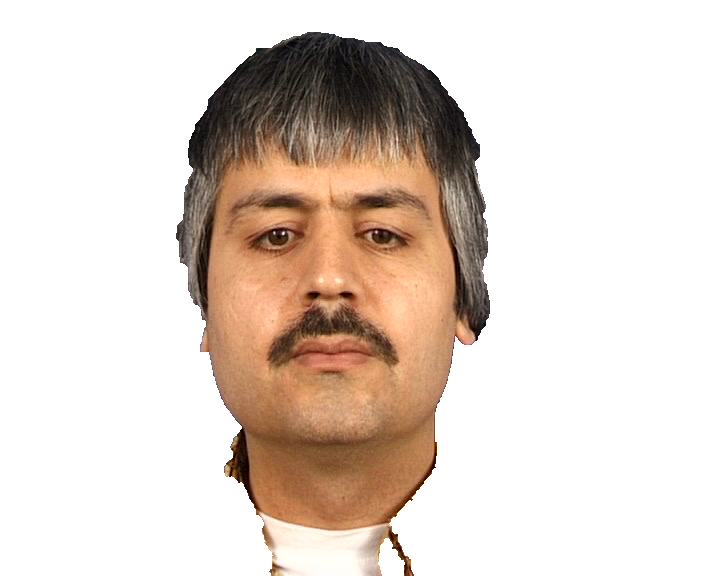
\includegraphics[width=0.2\linewidth]{018_4_2_masked}%
   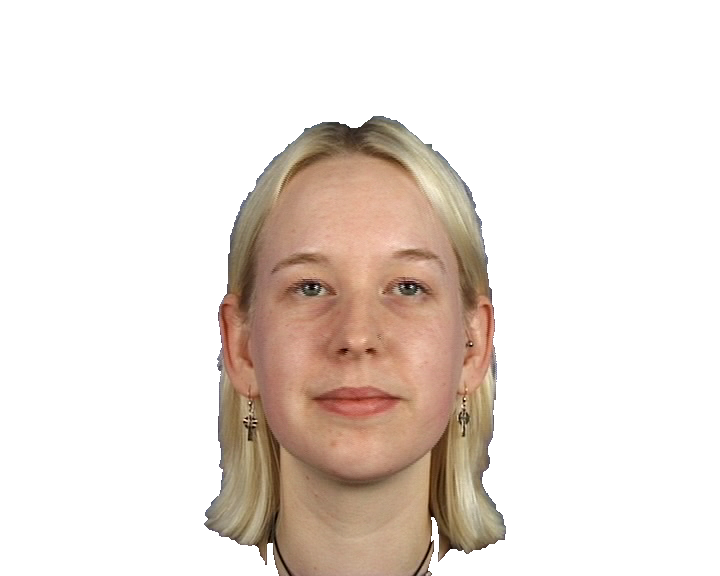
\includegraphics[width=0.2\linewidth]{328_2_1_masked}%
   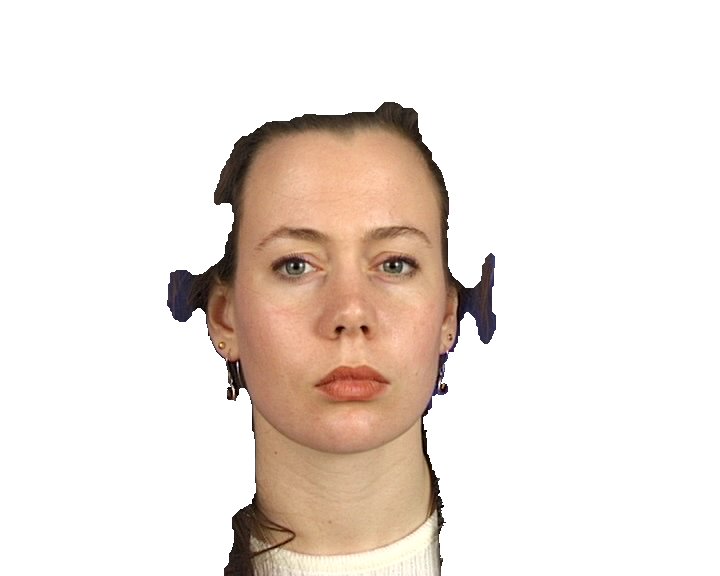
\includegraphics[width=0.2\linewidth]{319_2_1_masked}%
   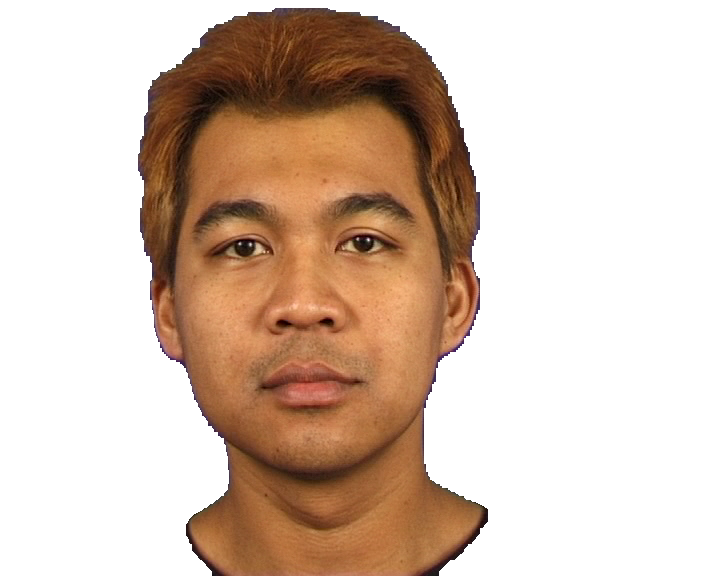
\includegraphics[width=0.2\linewidth]{027_4_2_masked}%
   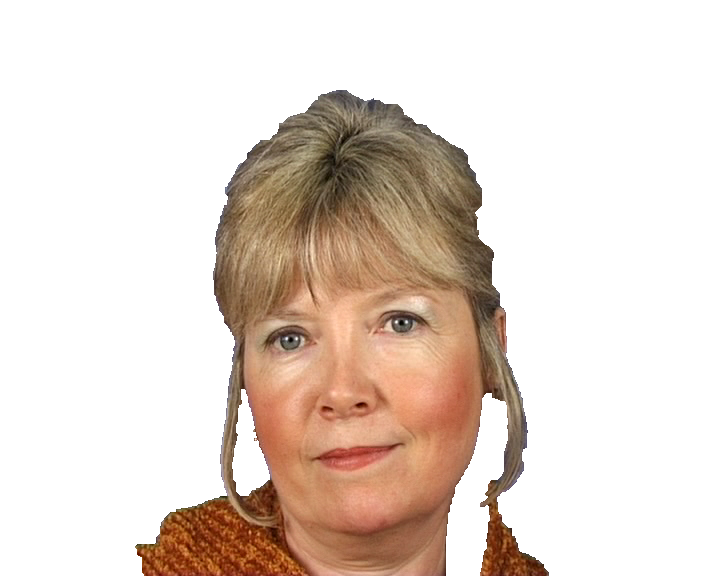
\includegraphics[width=0.2\linewidth]{020_1_1_masked}
   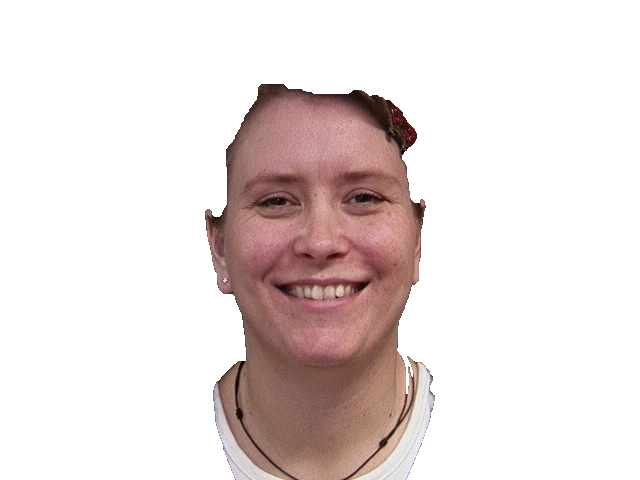
\includegraphics[width=0.2\linewidth]{12_2f_masked}%
   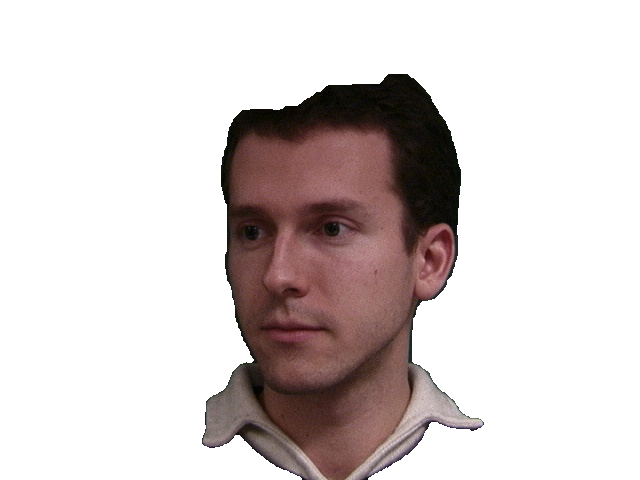
\includegraphics[width=0.2\linewidth]{21_3m_masked}%
   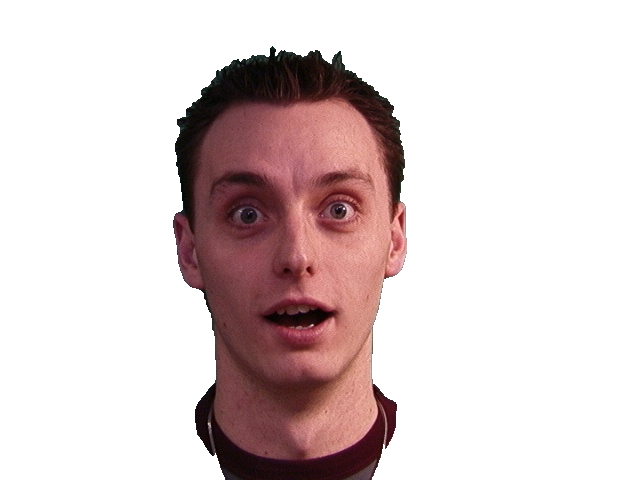
\includegraphics[width=0.2\linewidth]{09_6m_masked}%
   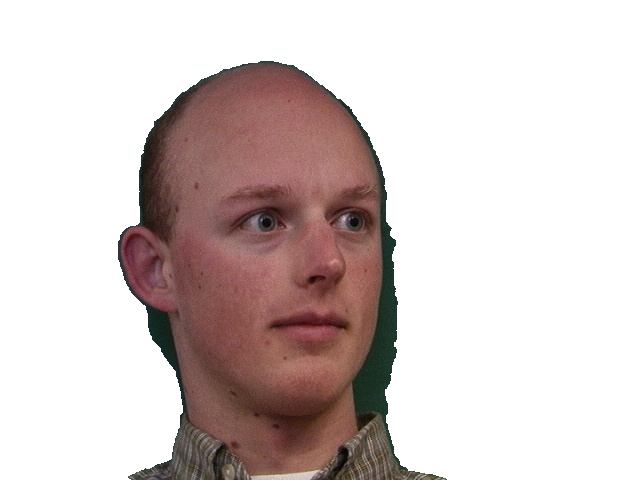
\includegraphics[width=0.2\linewidth]{33_4m_masked}%
   %\includegraphics[width=0.2\linewidth]{22_3f_masked}
   $\dots$\\
   The model was trained from 456 images from the IMM and XM2VTS datasets using
   120 landmarks. Get the landmarks, model, and source code at:\\
   \mbox{\url{www.cs.unibas.ch/personen/amberg_brian/aam/}}
   }

 %%%%%%%%%%%%%%%%%%%%%%%%%%%%%%%%%%%%%%%%%%%%%%%%%%%%%%%%%%%%%%%%%%%%%%%%%%%%%%

   \headerbox{Tracking 5000 frames with a general model}{name=tracking,column=2,span=2,below=speed,above=bottom}{
 %%%%%%%%%%%%%%%%%%%%%%%%%%%%%%%%%%%%%%%%%%%%%%%%%%%%%%%%%%%%%%%%%%%%%%%%%%%%%%
 {
 \begin{tabular}{c@{\hspace{0.05em}}c@{\hspace{0.1em}}c@{\hspace{0.1em}}c@{\hspace{0.1em}}c@{\hspace{1em}}c@{\hspace{0.1em}}c@{\hspace{0.1em}}c@{\hspace{0.1em}}c@{\hspace{0.1em}}c}
   \multicolumn{5}{c}{\smaller \ICIA{} with $\VLins$} &
   \multicolumn{5}{c}{\smaller \ICIA{} with $\VLins$ + Regularisation}\\[-0.2em]
   \includegraphics[width=0.095\linewidth]{track_frame_00010_01}&
   \includegraphics[width=0.095\linewidth]{track_frame_00050_01}&
   \includegraphics[width=0.095\linewidth]{track_frame_00450_01}&
   \includegraphics[width=0.095\linewidth]{track_frame_02000_01}&
   \includegraphics[width=0.095\linewidth]{track_frame_04999_01}&
   %
   \includegraphics[width=0.095\linewidth]{track_frame_00010_02}&
   \includegraphics[width=0.095\linewidth]{track_frame_00050_02}&
   \includegraphics[width=0.095\linewidth]{track_frame_00450_02}&
   \includegraphics[width=0.095\linewidth]{track_frame_02000_02}&
   \includegraphics[width=0.095\linewidth]{track_frame_04999_02}\\[-0.1em]
   %
   \multicolumn{5}{c}{\smaller \LinCoDe{}} &
   \multicolumn{5}{c}{\smaller \LinCoDe{} + Regularisation}\\[-0.2em]
   \includegraphics[width=0.095\linewidth]{track_frame_00010_03}&
   \includegraphics[width=0.095\linewidth]{track_frame_00050_03}&
   \includegraphics[width=0.095\linewidth]{track_frame_00450_03}&
   \includegraphics[width=0.095\linewidth]{track_frame_02000_03}&
   \includegraphics[width=0.095\linewidth]{track_frame_04999_03}&
   %
   \includegraphics[width=0.095\linewidth]{track_frame_00010_04}&
   \includegraphics[width=0.095\linewidth]{track_frame_00050_04}&
   \includegraphics[width=0.095\linewidth]{track_frame_00450_04}&
   \includegraphics[width=0.095\linewidth]{track_frame_02000_04}&
   \includegraphics[width=0.095\linewidth]{track_frame_04999_04}\\[-0.1em]
   %
   \multicolumn{5}{c}{\smaller \CoDe{}} &
   \multicolumn{5}{c}{\smaller \CoDe{} + Regularisation}\\[-0.2em]
   \includegraphics[width=0.095\linewidth]{track_frame_00010_05}&
   \includegraphics[width=0.095\linewidth]{track_frame_00050_05}&
   \includegraphics[width=0.095\linewidth]{track_frame_00450_05}&
   \includegraphics[width=0.095\linewidth]{track_frame_02000_05}&
   \includegraphics[width=0.095\linewidth]{track_frame_04999_05}&
   %
   \includegraphics[width=0.095\linewidth]{track_frame_00010_06}&
   \includegraphics[width=0.095\linewidth]{track_frame_00050_06}&
   \includegraphics[width=0.095\linewidth]{track_frame_00450_06}&
   \includegraphics[width=0.095\linewidth]{track_frame_02000_06}&
   \includegraphics[width=0.095\linewidth]{track_frame_04999_06}\\[-0.5em]
   \smaller Frame 10 & \smaller Frame 50 & \smaller Frame 450 & \smaller Frame 2000 & \smaller Frame 5000 &
   \smaller Frame 10 & \smaller Frame 50 & \smaller Frame 450 & \smaller Frame 2000 & \smaller Frame 5000
   \end{tabular}
 }
   \vspace{-1.2em}
   \begin{multicols}{2}
   {\textbf{Our algorithm makes fast and robust tracking possible.}
     We compare face tracking under natural motion, using \ICIA{},
     \LinCoDe{} and \CoDe{}. The original \ICIA{} fails
     immediately with this large model and new face data. Substituting the orthonormal
     incremental warp for the original \ICIA{} warp, the algorithm still loses track
     very early, whereas \LinCoDe{} and \CoDe{} can track much
     further. Finally, adding regularisation to all algorithms, \ICIA{} still
     loses track completely after approximately 500 frames and does not recover
     the local deformations accurately. In contrast \CoDe{} now tracks the full
     5000 frame sequence without reinitialization, and \LinCoDe{} tracks for 2500 frames.}
   
   The same training dataset was used for both tracking experiments. The
   training data was aquired with different camera and light settings from
   different subjects.
   \end{multicols}
   }
 %%%%%%%%%%%%%%%%%%%%%%%%%%%%%%%%%%%%%%%%%%%%%%%%%%%%%%%%%%%%%%%%%%%%%%%%%%%%%%
   \headerbox{Low Res Tracking}{name=lowrestracking,column=1,span=1,below=speed,above=bottom}{
 %%%%%%%%%%%%%%%%%%%%%%%%%%%%%%%%%%%%%%%%%%%%%%%%%%%%%%%%%%%%%%%%%%%%%%%%%%%%%%
\begin{tabular}{@{}c@{}c@{}c@{}c@{}c@{}}
  \multicolumn{5}{c}{\smaller \ICIA{} with $\VLins$}\\[-0.2em]
  \includegraphics[width=0.2\linewidth]{bush_00010_02}&
  \includegraphics[width=0.2\linewidth]{bush_00100_02}&
  \includegraphics[width=0.2\linewidth]{bush_00200_02}&
  \includegraphics[width=0.2\linewidth]{bush_00300_02}&
  \includegraphics[width=0.2\linewidth]{bush_00400_02}\\[-0.1em]
  \multicolumn{5}{c}{\smaller \LinCoDe{}}\\[-0.2em]
  \includegraphics[width=0.2\linewidth]{bush_00010_05}&
  \includegraphics[width=0.2\linewidth]{bush_00100_05}&
  \includegraphics[width=0.2\linewidth]{bush_00200_05}&
  \includegraphics[width=0.2\linewidth]{bush_00300_05}&
  \includegraphics[width=0.2\linewidth]{bush_00400_05}\\[-0.1em]
  \multicolumn{5}{c}{\smaller \CoDe{}}\\[-0.2em]
  \includegraphics[width=0.2\linewidth]{bush_00010_08}&
  \includegraphics[width=0.2\linewidth]{bush_00100_08}&
  \includegraphics[width=0.2\linewidth]{bush_00200_08}&
  \includegraphics[width=0.2\linewidth]{bush_00300_08}&
  \includegraphics[width=0.2\linewidth]{bush_00400_08}\\[-0.5em]
  \smaller Frame 10 & \smaller Frame 100 & \smaller Frame 200 & \smaller Frame 300 & \smaller Frame 400 
  \end{tabular}

  \vspace{1.25em}
  \textbf{Tracking a low resolution video with large head motions
  succeeds with \CoDe{}, where \ICIA{} fails.}\\ All methods used the orthonormal
  incremental warp, and relatively strong regularisation.  \ICIA{} starts to
  drift in the early frames, while~\CoDe{} tracks the full sequence. The
  approximate gradient method \LinCoDe{} also suceeds, but looses
  track of the details for about 100 frames.
   }

 %%%%%%%%%%%%%%%%%%%%%%%%%%%%%%%%%%%%%%%%%%%%%%%%%%%%%%%%%%%%%%%%%%%%%%%%%%%%%%%
  \headerbox{Compositional Alignment}{name=algorithm,column=1,above=lowrestracking,below=contribution}{
 %%%%%%%%%%%%%%%%%%%%%%%%%%%%%%%%%%%%%%%%%%%%%%%%%%%%%%%%%%%%%%%%%%%%%%%%%%%%%%%
  \begin{algorithm}[H]
    \dontprintsemicolon
    \linesnumbered
    \For{Blur and regularisation values}{
      \nl Initialize $\qq, \qq_{\text{best}}$ and $\kappa$\;
      \Repeat{converged}{
        \nl Calculate $\Nabla{\pp}{\tilde{F}(\qq,\VEC 0)}$, $F(\qq)$\;
        \eIf{$F(\qq) < F(\qq_{\text{best}})$}{
          %\nl Calculate distance between best warp estimate and current warp estimate to test for convergence\;
          \nl $\qq_{\text{best}} \gets \qq$\;
          %\If{More than three successiv updates}{ (Too much detail)
            \nl Increase $\kappa$\;
          %}
        }{
          \If{$\kappa$ smaller than threshold}{
            \nl return\;
          }%{
             decrease $\kappa$\;
          %}
        }
        \nl Calculate $\pp$ from $\Nabla{\pp}{\tilde{F}(\qq_{best},\pp)}$ and $\kappa$\;
        \nl $\qq \gets \C{\circ}{\qq, \pp}$
      }
    }
  \end{algorithm}
   }
\end{poster}%
%
\end{document}
